\chapter{Versuchsaufbau und -ablauf}\label{Kap3}

Das folgende Kapitel beschreibt Versuchsaufbau und -durchf"uhrung sowie Ziele der Messung, von der Erkenntnisse "uber das Skalierungsverhalten eines RPi-Clusters unter der Arbeitslast der ausgew"ahlten HPC-Benchmarks erwartet werden. 

\section{Zielsetzung}\label{Ziel}

F"ur das Skalierungsverhalten des Bramble unter der Arbeitslast von Linpack und STREAM werden wie in Kap. \ref{Kap2} beschrieben zwei Ma\ss zahlen betrachtet: Performance und Energieverbrauch.

Die augew"ahlten Benchmarks werden auf n -- 1 RPi-Knoten des Bramble mit n=19 RPi-Nodes ausgef"uhrt (vgl. Kap. \ref{Versuchsaufbau}). Alle Messungen werden zweimal durchgef"uhrt: Mit Stromanschluss der nicht beteiligten RPi-Nodes und ohne. F"ur beide Benchmarks werden zwei Ergebnisparameter betrachtet: Ausf"uhrungsrate in GFLOPs und Ausf"uhrungszeit in s f"ur HPLinpack, Ausf"uhrungsrate in MB/s und durchschnittliche Ausf"uhrungszeit in s f"ur STREAM. Die Ergebnisse der Messreihen werden anschlie\ss end gegen"ubergestellt (vgl. Kap. \ref{Ergebnisse}). 

\section{Aufbau und Art der Messung}\label{Aufbau}

Hier stellen sich zwei grunds"atzliche Fragen: Welcher Art ist die Messung und welche Voraussetzungen m"ussen hierf"ur erf"ullt sein? 

Die Performance wird pro Benchmark durch zwei Ergebnisparameter ermittelt. Zwei Messreihen werden durchgef"uhrt: Bramble mit n RPi-Knoten aktiv/20 RPi-Knoten angeschaltet, Bramble mit n RPi-Knoten aktiv/n RPi-Knoten angeschaltet. 
% TODO: evtl. bessere Einleitung/Herleitung 
F"ur den Versuchsaufbau sind folgende Aspekte von Bedeutung: M"ogliche Modifikationen der RPi-Knoten, Zeitsynchronisation der RPi-Knoten, Skalierung der Messung auf n -- 1 RPi-Knoten, automatisierte Durchf"uhrung der Messung auf n -- 1 RPi-Knoten sowie Einlesen der Messwerte in eine geeignete Datenstruktur. 

\subsection{Versuchsaufbau Ri-Einzelrechner}\label{RPi-Versuchsaufbau}

Viele Nutzer stellen sich nach Inbetriebnahme eines RPi-Einzelrechners die Frage nach Swap-Speicher und "Ubertakten (vgl. \cite{pow12}). Beides liegt nahe, da das Modell B des RPi nur "uber 512 MB Arbeitsspeicher verf"ugt. Die CPU-Leistung ist mit 700 MHz ebenfalls eher niedrig. 

Im Praxisbetrieb wurde gezeigt, dass ein "Ubertakten der CPU auf bis zu 1 GHz gefahrlos m"oglich ist (vgl. z.B. \url{http://www.raspberrypi.org/introducing-turbo-mode-up-to-50-} \url{more-performance-for-free/}). Bei den hier verwendeten RPis wurde davon Abstand genommen, da es wenig zielf"uhrend erscheint, die Komponente zu manipulieren, deren Performance man durch Benchmarking evaluieren m"ochte\footnote{F"ur eine zuk"unftige Untersuchung w"are es interessant zu ermitteln, ob man den relativ hohen Stromverbrauch des Bramble bei Niedriglast (vgl. \cite{kli13}) durch Untertakten der einzelnen CPUs senken kann (vgl. Kap. \ref{Kap5}).} Allerdings gibt es bereits Ergebnisse f"ur Linpack 100 und Whetstone bei auf einem RPi-Einzelrechner bei "Ubertakten der CPU auf 1 MHz (vgl. \url{http://www.roylongbottom.org.uk/Raspberry\%20Pi\%20Benchmarks.htm}).

Zur Allokierung von Swap-Speicher auf dem RPi gibt es grunds"atzlich drei M"oglichkeiten: Swap-Datei, Swap-Partition oder zRAM. 

Das Betriebssystem Raspbian verwendet standardm"a\ss ig eine Swap-Datei \texttt{/var/swap} auf der SD-Karte (vgl. \url{http://raspberrypi.stackexchange.com/questions/70/how-to-set} \url{-up-swap-space}). Hierbei zeigen sich Probleme: Erstens k"onnen st"andige Schreibzugriffe auf Dauer die SD-Karte besch"adigen. Zweitens sind Schreibzugriffe darauf sehr langsam, was die Performance des Systems bei hoher Arbeitsspeicherlast beeintr"achtigen kann (vgl. \cite{pow12}). 

Das gilt auch f"ur die Allokierung einer auf Unix-Systemen "ublicherweise genutzten Swap-Partition, weswegen diese M"oglichkeit in der Praxis keine Rolle spielt. 

Eine weitere M"oglichkeit des Swapping ist die Verwendung von zRAM. Hierbei wird ein Teil des Arbeitsspeichers komprimiert und als Swap Space genutzt. Hierbei werden keine Zugriffe auf die SD-Karte notwendig (vgl. \cite{pow12}). 

% Die Swap-Datei kann mit dem Befehl \texttt{sudo update-rc.d dphys-swapfile remove} deaktiviert werden. 
Auf dem Bramble-Server war kein Swap-Speicher allokiert worden (vgl. \cite{kli13}). Trotz der beschriebenen Schwierigkeiten wird auf den RPi-Knoten ein gro\ss er Teil des Speichers auf den SD-Karten als Swap-Speicher genutzt, um die Nutzung von Programmen mit mehr Speicherbedarf zu erm"oglichen und das Netzwerk durch das Cachen h"aufig verwendeter Dateien zu entlasten (vgl. \cite{kli13}).  

\subsection{Versuchsaufbau Bramble}\label{Bramble-Versuchsaufbau}

Das Komponentendiagramm \ref{fig:Komponentendiagramm} zeigt den Versuchsaufbau pro Messreihe auf dem Bramble mit Stromversorgung, Netzanschluss und Strommessger"at als phyischen Komponenten und der MySQL-Datenbank als logischer Komponente. Eine Messreihe wird als \textit{ExperimentSuite} bezeichnet. 
\begin{figure}[htb]
  \centering
  \centerline{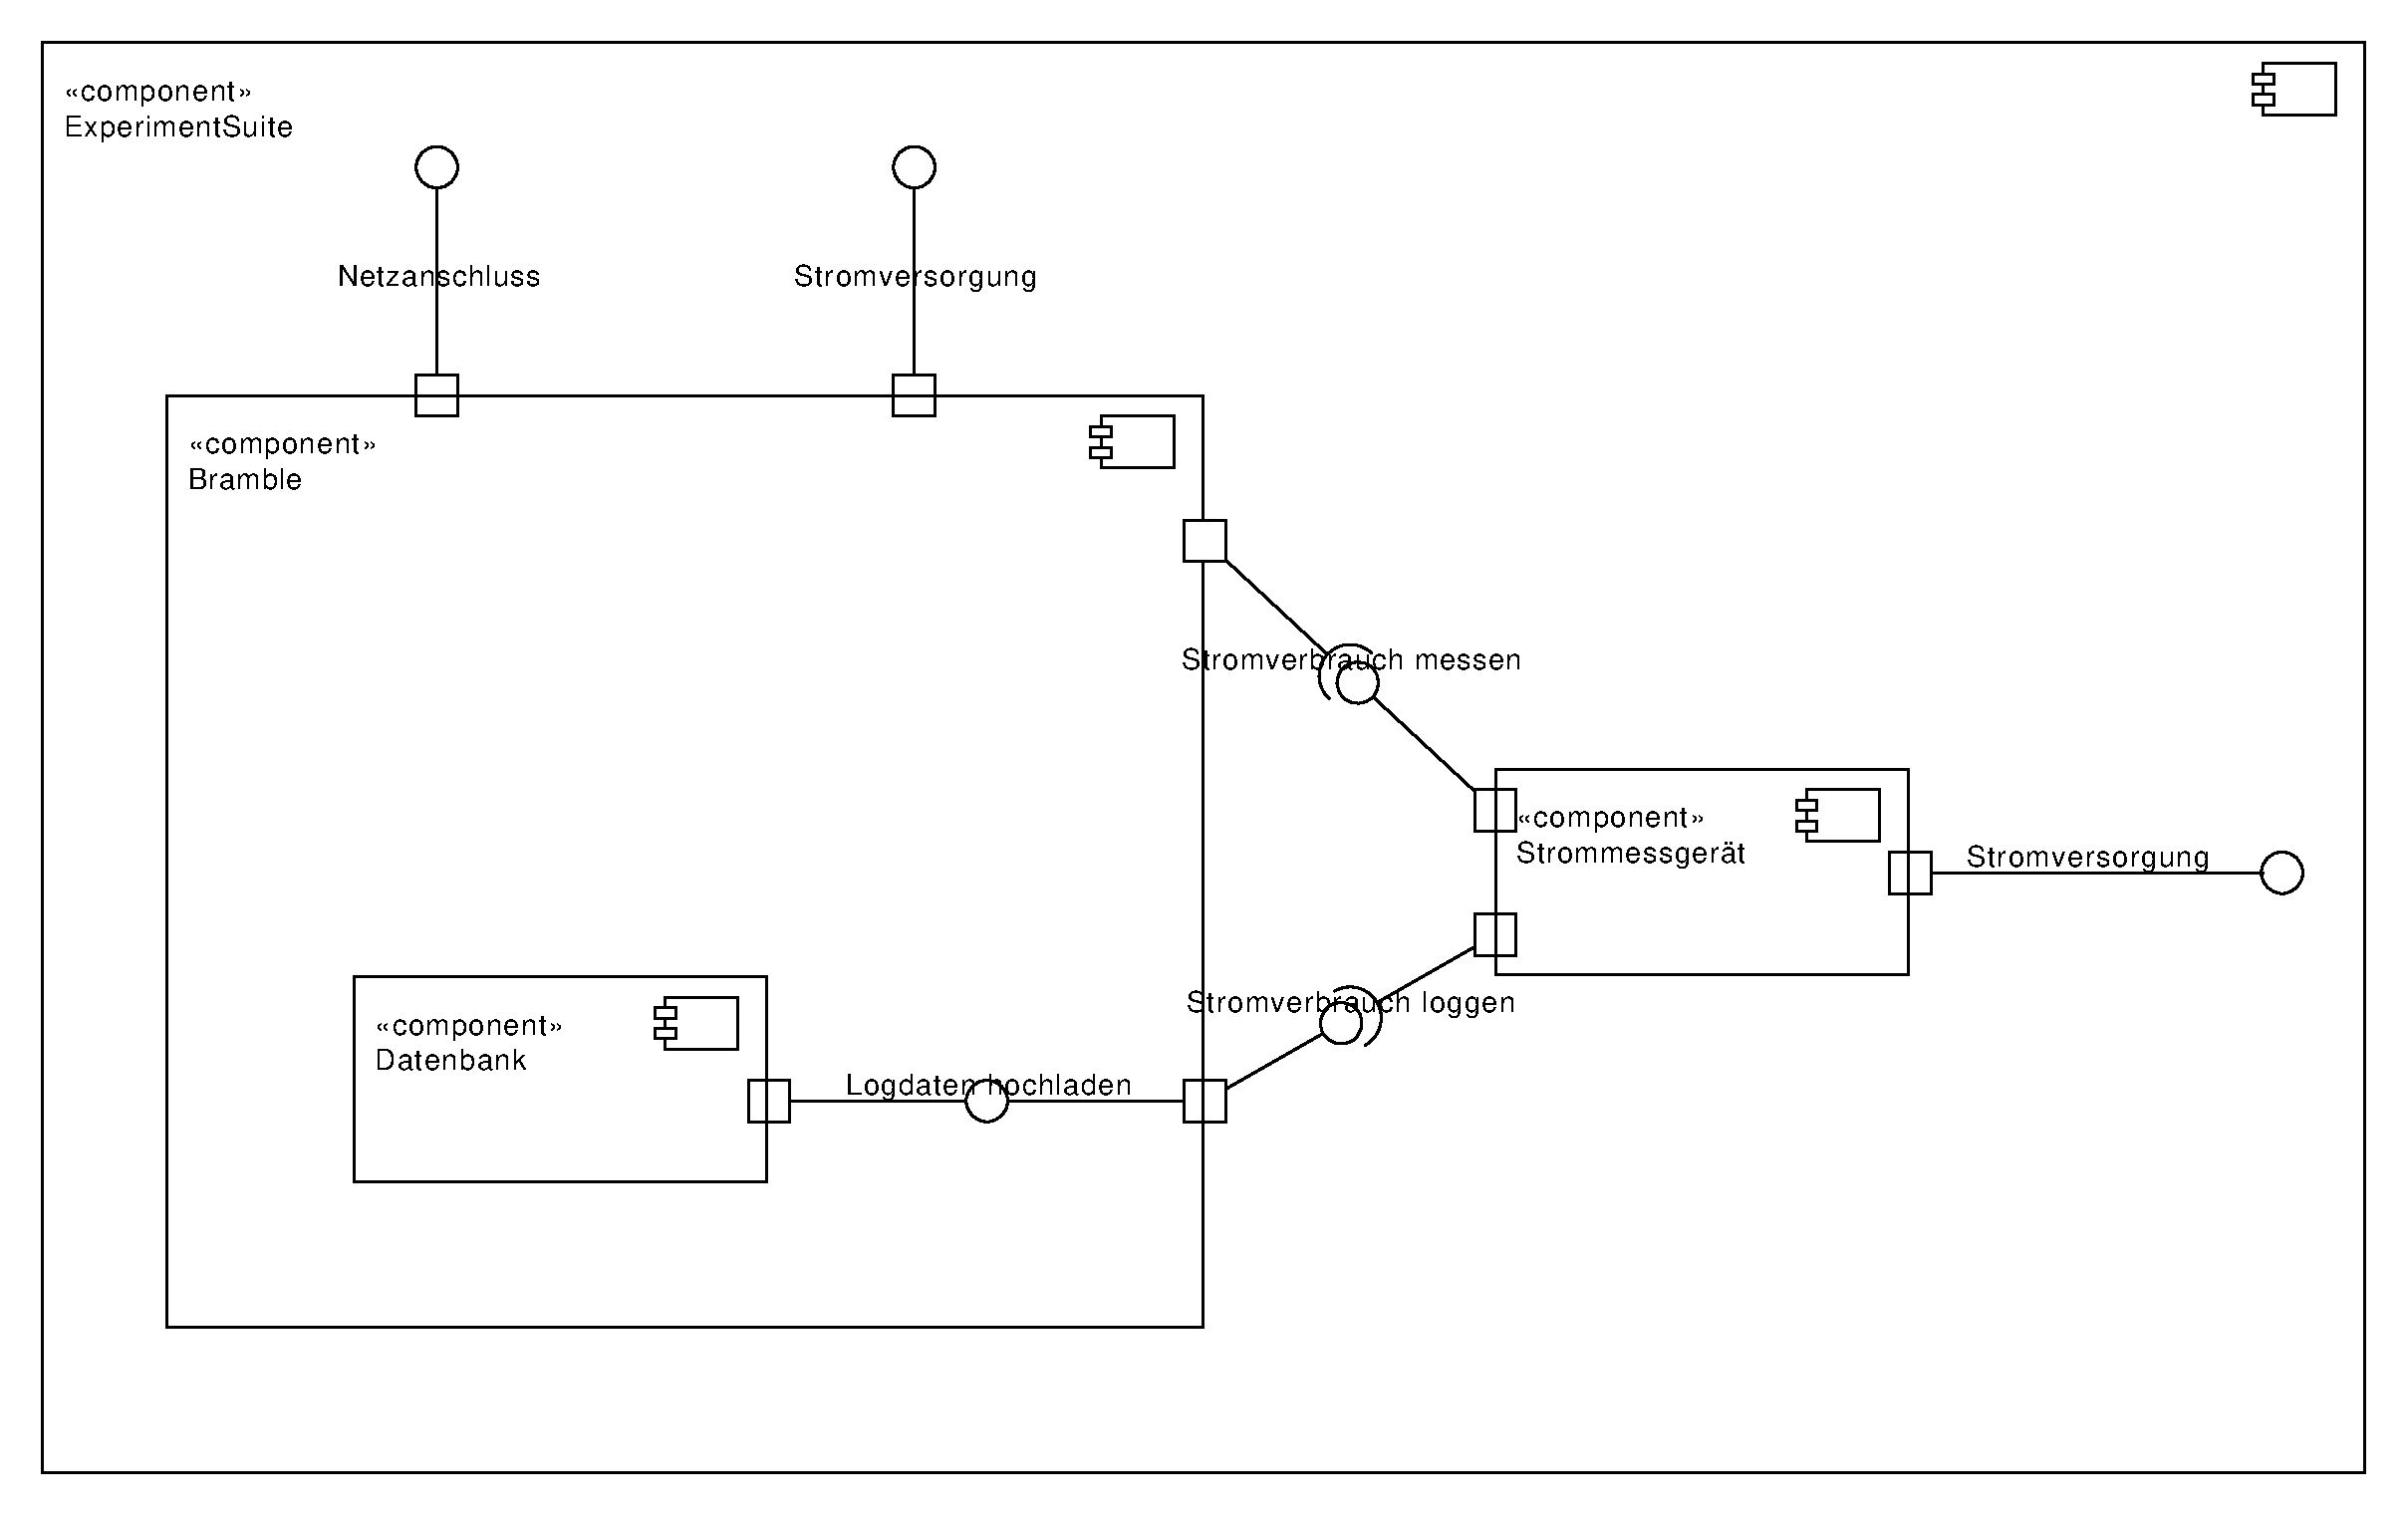
\includegraphics[scale=0.5]{komponentendiagramm2.pdf}} 
  \caption{Komponentendiagramm des Versuchsaufbaus.}
  \label{fig:Komponentendiagramm}		
\end{figure}
\subsubsection{Modifikation der RPi-Knoten}

Zu Beginn der Untersuchung zeigte sich, dass bei einige Mini-USB-Kabel zur Stromversorgung der RPis einen Wackelkontakt hatten oder ganz defekt waren. Um die in Kap. \ref{Vorgehensweise} genannte Zuverl"assigkeit des Versuchsaufbaus sicherzustellen, wurden sie durch funktionsf"ahige Kabel ersetzt. 

\subsubsection{Zeitsynchronisation der RPi-Knoten} 

Der RPi-Einzelrechner besitzt aus Kostengr"unden keine Systemuhr (vgl. \cite{schmi13}), sondern synchronisiert sich beim Booten gegen einen NTP-Server im Internet. F"ur die parallele Ausf"uhrung eines Programms auf mehreren Rechnerkernen ist die Zeitsynchronisation der RPi-Knoten und des Servers essentiell. Auf dem Bramble-Server gibt es daher einen OpenNTP-Server, gegen den sich die RPi-Knoten synchronisieren (vgl. \cite{kli13}). 

\subsubsection{Skalierung der Messung auf n -- 1 RPi-Knoten} 

Das Aktivit"atsdiagramm \ref{fig:Aktivitaetsdiagramm} zeigt, welche Schritte aus Benutzersicht f"ur die Durchf"uhr\-ung einer ExperimentSuite, d.h. der Ausf"uhrung eines Benchmarks auf einer gew"ahlten Anzahl aktiver und angeschalteter RPi-Knoten erforderlich sind. Es wird mit n=19 RPi-Knoten begonnen und einmal "uber alle Knoten von 19 -- 1 (ohne den Ausf"uhrungsknoten \texttt{pi03}) iteriert. Danach wird die zweite Messung durchgef"uhrt, wobei nach jedem Iterationsschritt der nicht mehr ben"otigte RPi-Knoten abgeschaltet wird. Jede Iteration der Benchmark-Ausf"uhrung l"auft prinzipell gleich ab, w"ahrend am Anfang und am Ende spezielle Vorkehrungen zu treffen sind. 
\begin{figure}[htb]
  \centerline{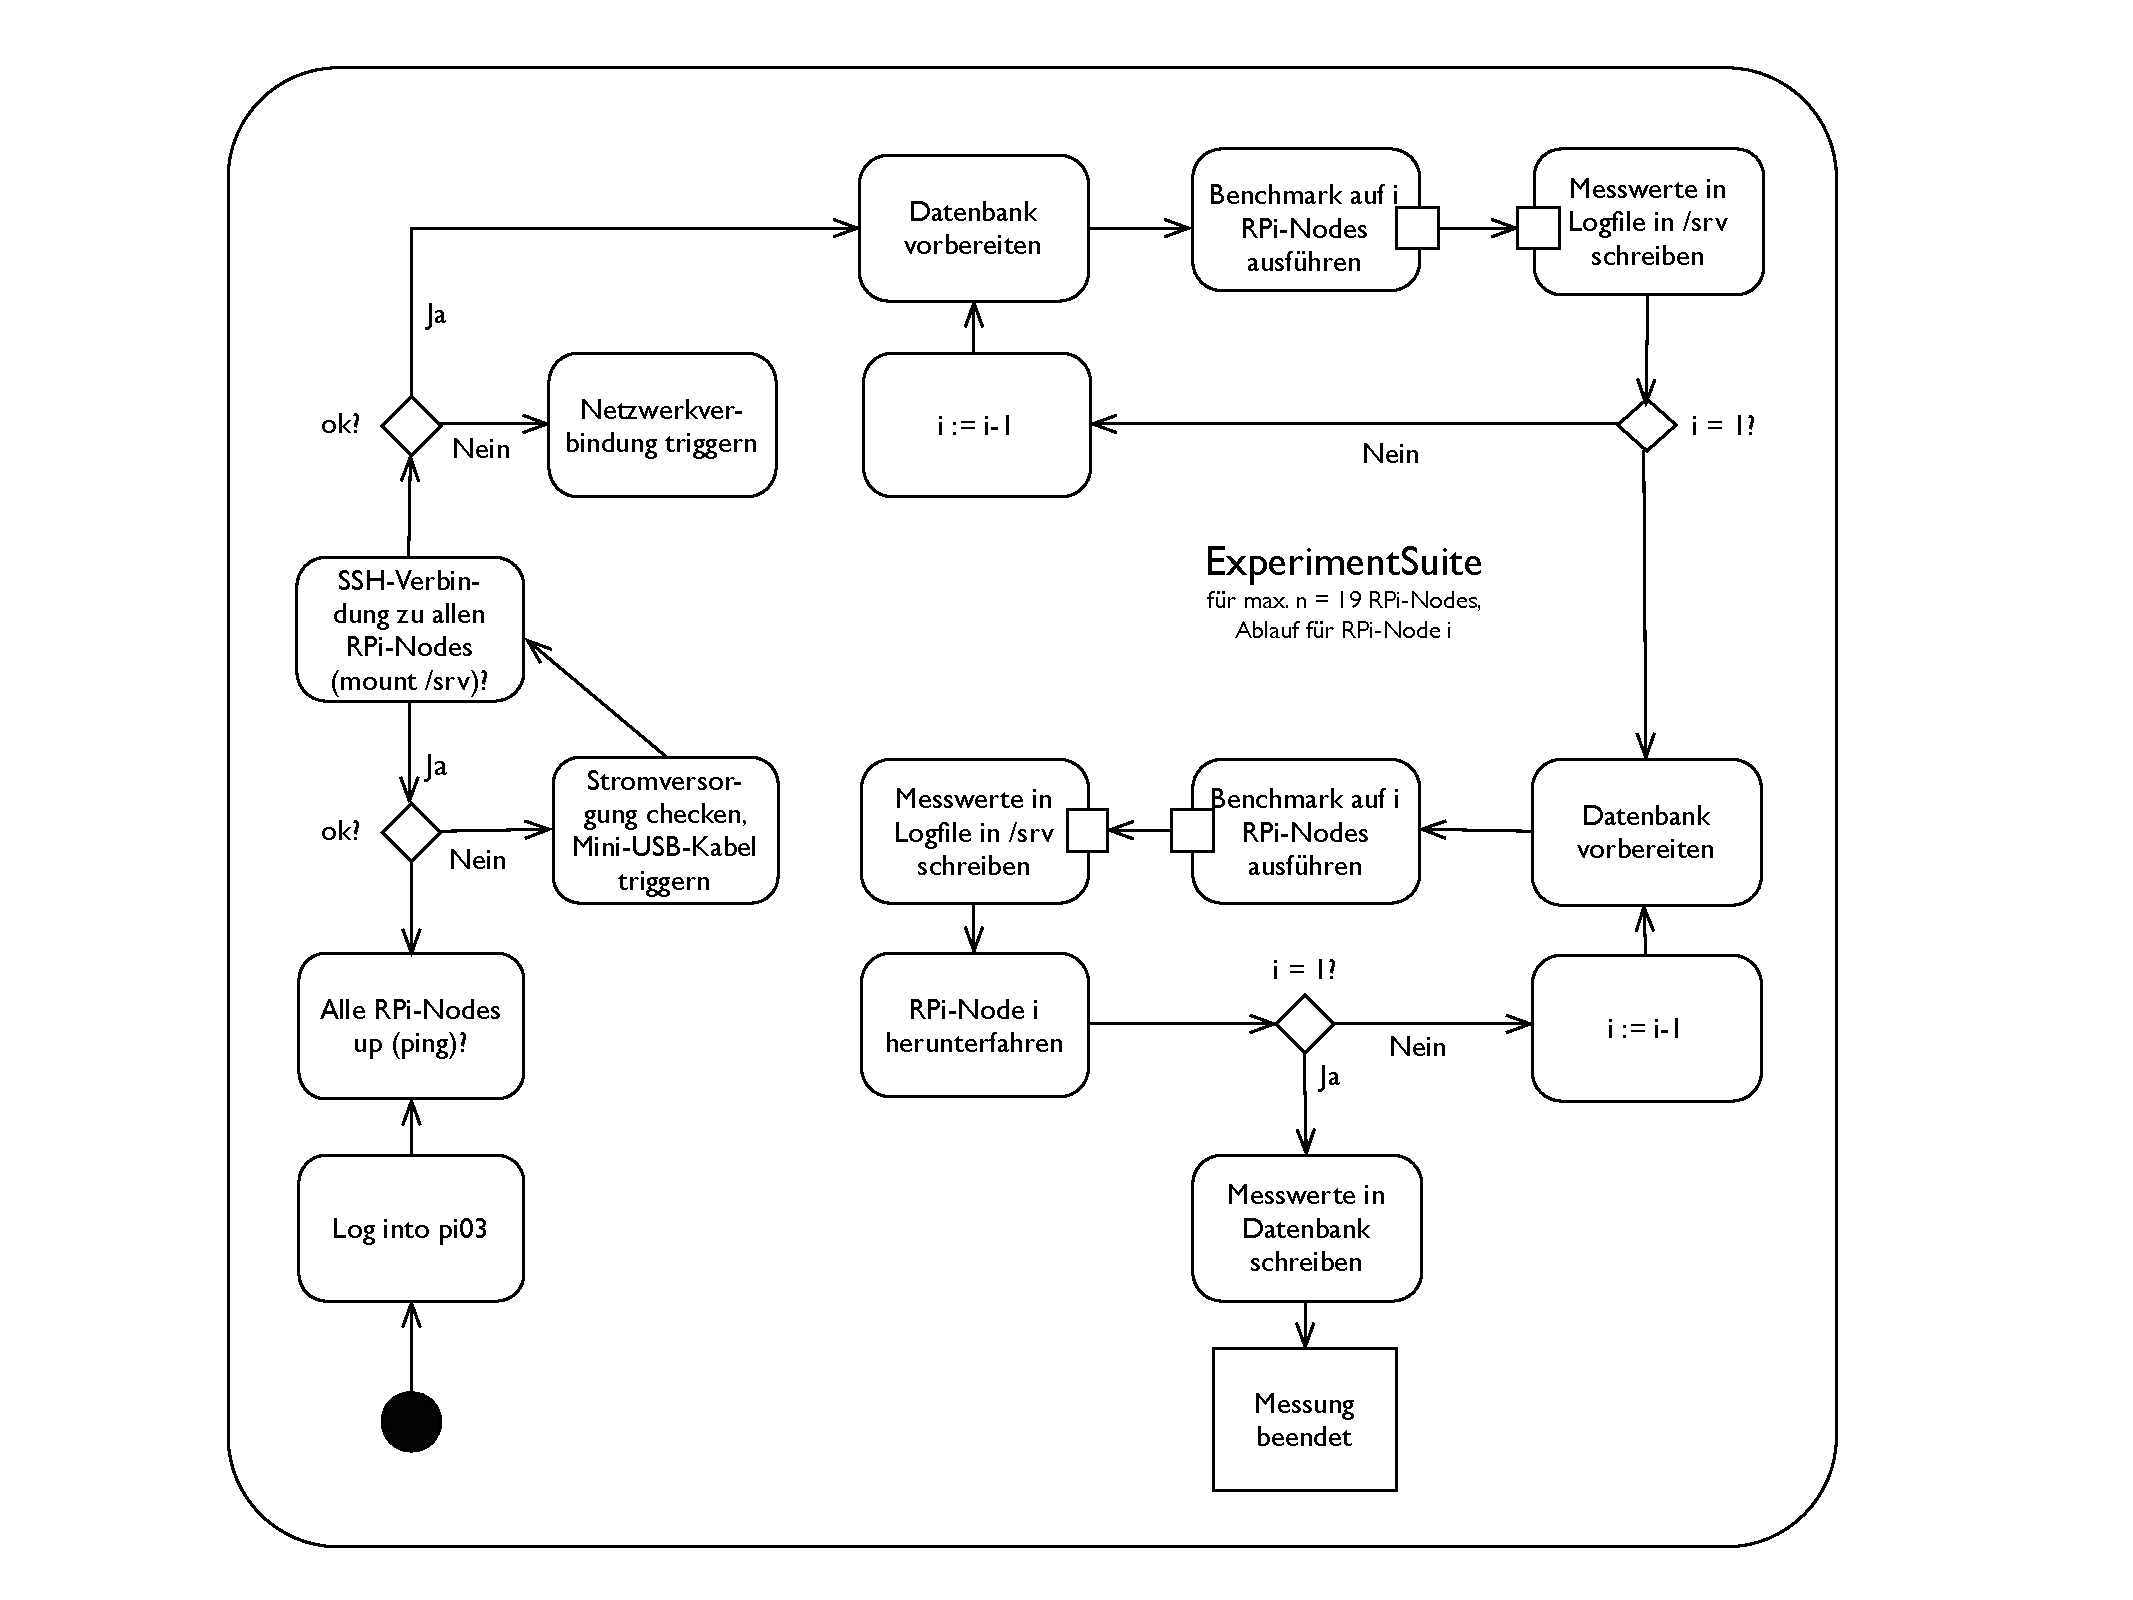
\includegraphics[scale=0.5]{aktivitaetsdiagramm1.pdf}} 
  \caption{Aktivit"atsdiagramm einer ExperimentSuite.}
  \label{fig:Aktivitaetsdiagramm}
\end{figure}

\subsubsection{Konfiguration der Datenbank}

Die Konfigurationen der Benchmarks und der ExperimentSuites sowie die Messergebnisse der Benchmarks werden in einer MySQL-Datenbank auf \texttt{careme} abgelegt. Daf"ur war ein Datenbankschema vorgegeben worden, das die Bramble-ExperimentSuites in einen gr"o\ss eren Versuchsaufbau integriert. W"ahrend der praktischen Arbeit wurde das Schema geringf"ugig an die tats"achlichen Erfordernisse angepasst. Z.B. wurde f"ur jedes ausgef"uhrte Teilmodul eines Benchmarks ein Messpaarameter definiert, der Unix-Timestamp seines Ausf"uhrungsendes ermittelt und zusammen mit dem jeweiligen Messwert in die Datenbank eingelesen.

Die Vorbereitung der Datenbank f"ur den Versuchaufbau erfolgt in vier Schritten:  
\begin{enumerate}\bfseries
	\item Name und Beschreibung des Benchmarks. 
	\item Beschreibung des Versuchsaufbaus. 
	\item Konfiguration des Versuchsaufbaus. 
	\item Verkn"upfung von Benchmark-Konfiguration und Versuchsaufbau.
\end{enumerate} 
Das Aktivit"atsdiagramm \ref{fig:Dbconfig1} visualisiert Schritt 1. Hier werden die statischen Konfigurationen f"ur STREAM und HPLinpack festgelegt, was durch zwei Shellskripte \texttt{loadGeneratorCon\-figHpl.sh} und \texttt{loadGenerator\-ConfigStream.sh} realisiert wird. Sie werden zu Beginn des Versuchs einmal ausgef"uhrt. Pro Benchmark muss in drei Tabellen jeweils ein Eintrag erstellt werden: In der Tabelle \texttt{LoadGenerator} muss ein Eintrag mit Werten f"ur Name und Beschreibung des Benchmarks eingegeben werden. In der Tabelle \texttt{ENUM\_LoadGeneratorConfigura\-tionKey} muss Eintrag mit einem Wert f"ur den Konfigurationsschl"ussel des Benchmarks erstellt werden. In der Tabelle \texttt{LoadGeneratorConfiguration} muss ebenfalls ein Eintrag mit diesem Wert erstellt werden.
\begin{figure}[htb]
\centering
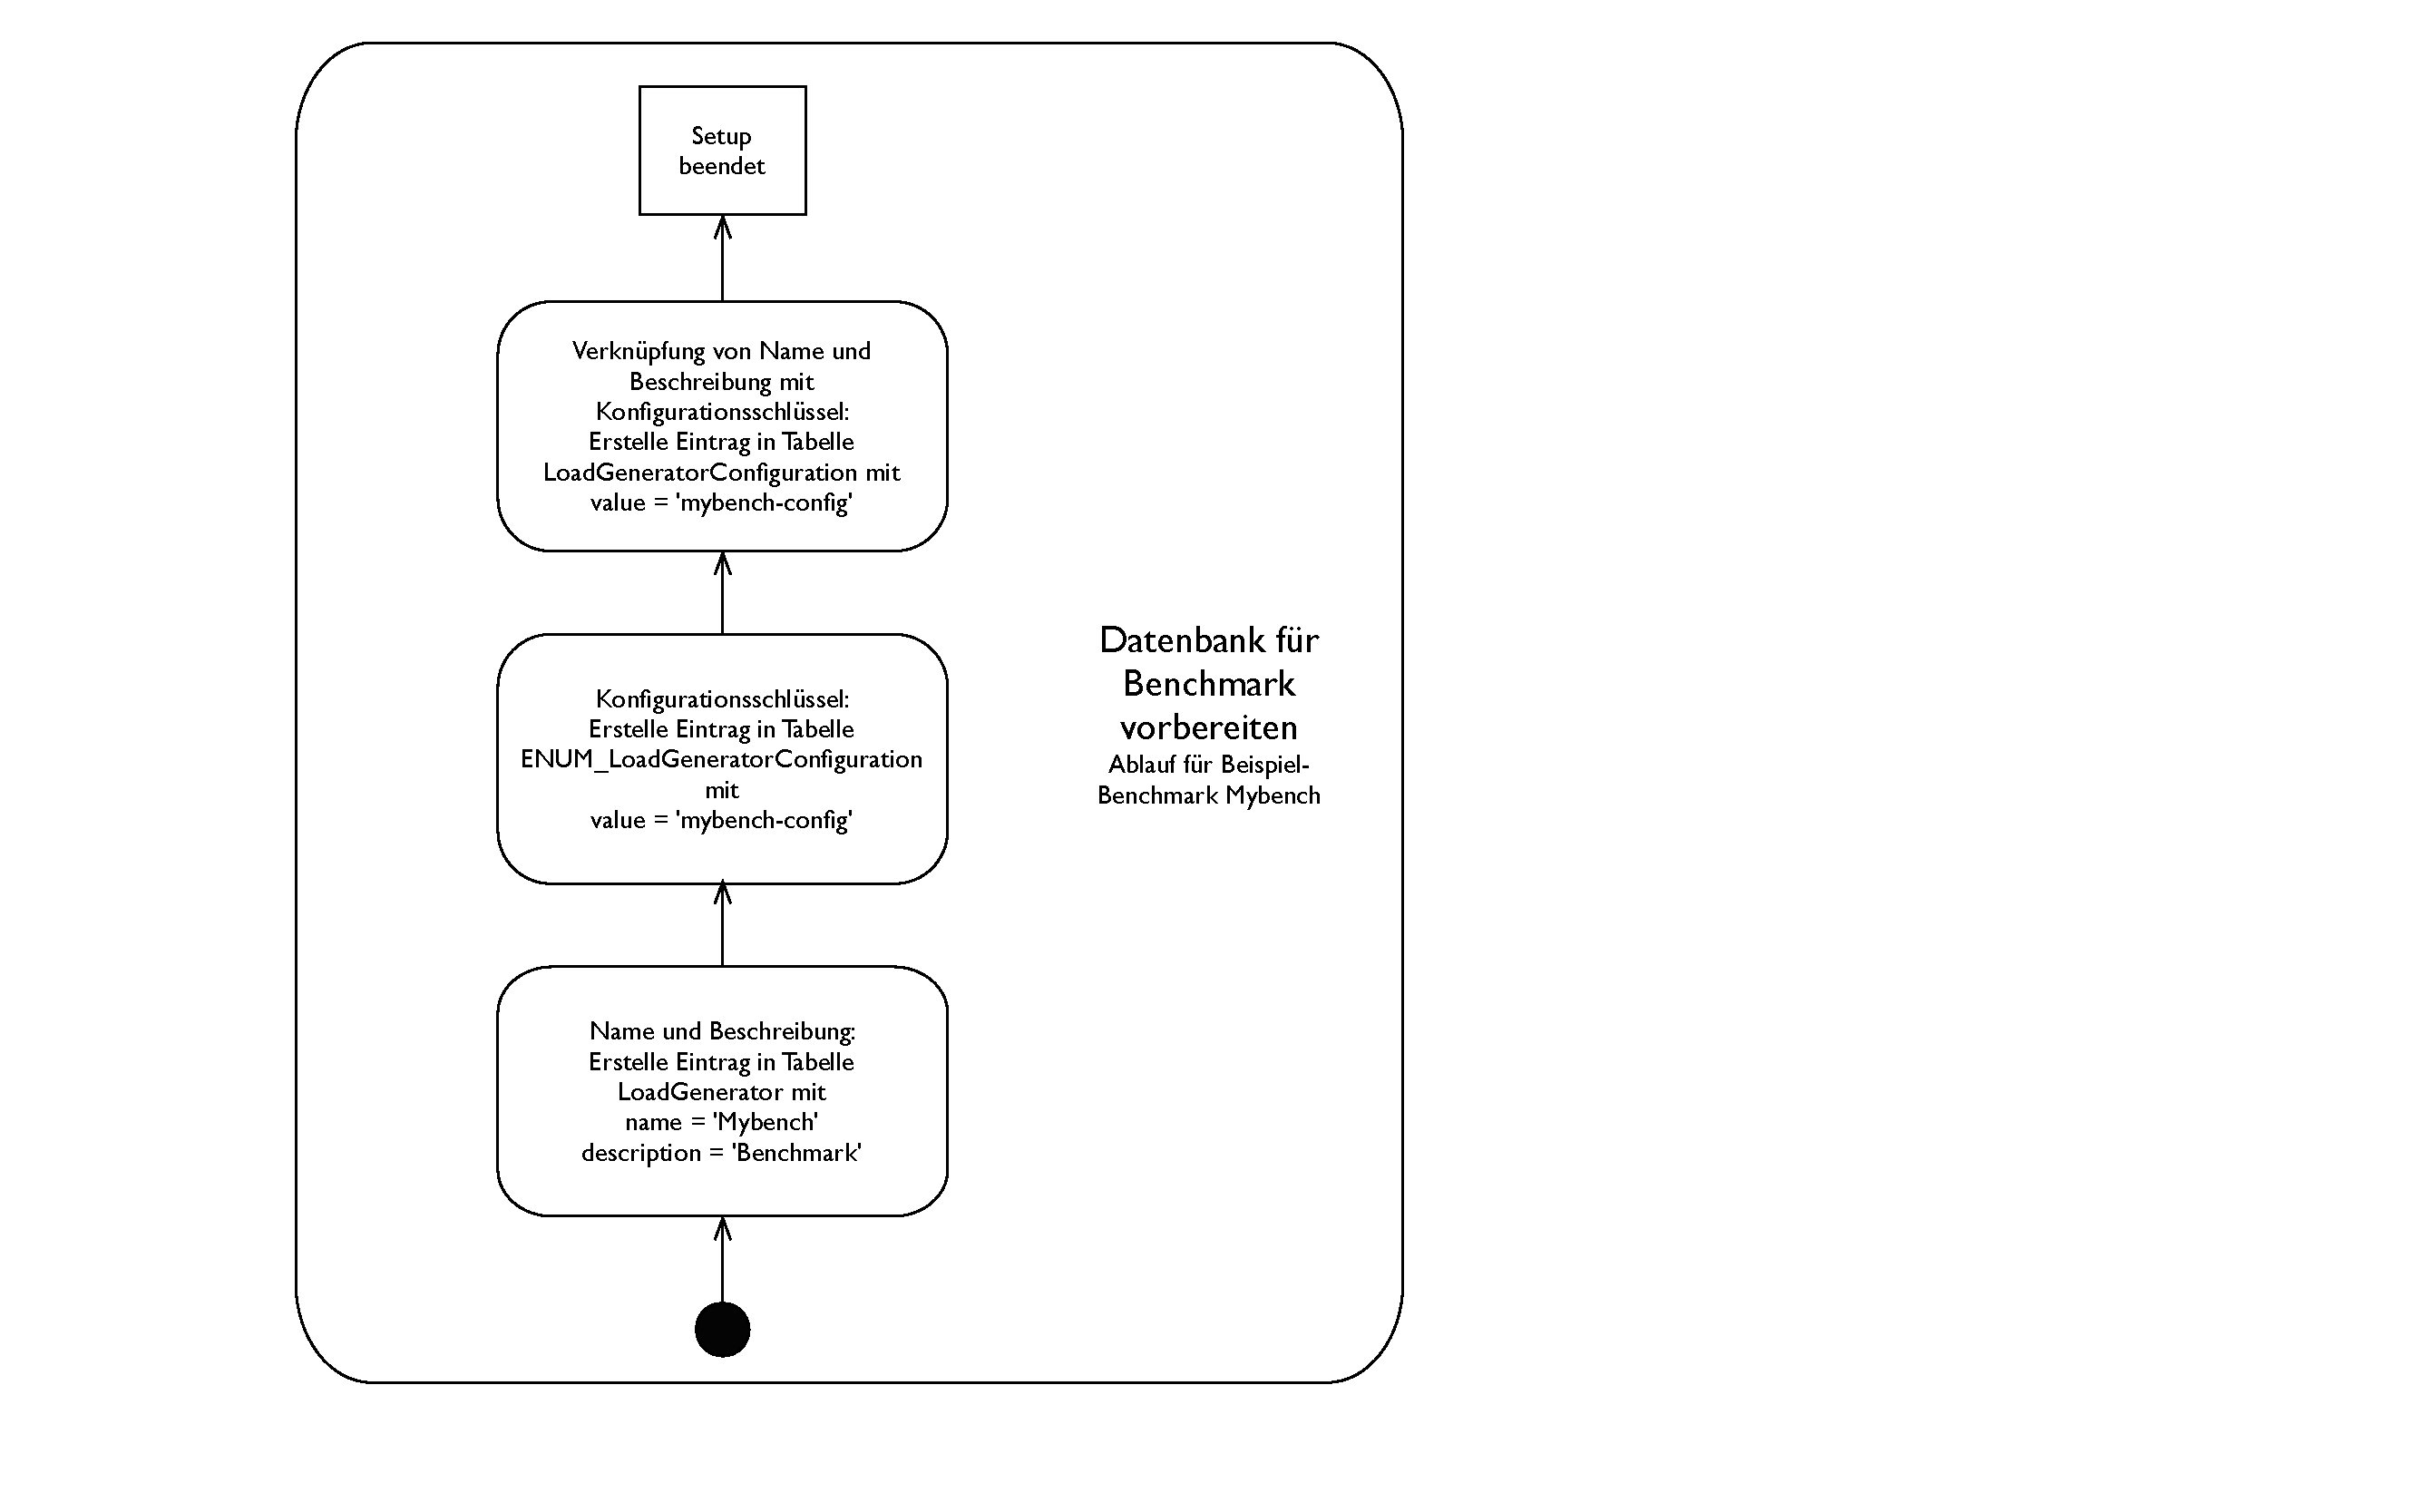
\includegraphics[scale=0.5]{dbconfig1.pdf}
\caption{Aktivit"atsdiagramm zur Vorbereitung der Datenbank f"ur einen Benchmark.}
\label{fig:Dbconfig1}
\end{figure}
Die dynamischen Schritte 2 -- 4, die pro ExperimentSuite ausgef"uhrt werden (Name, Beschreibung und Konfiguration des Versuchsaufbaus sowie Verkn"upfung von ExperimentSuite und Benchmark-Konfiguration) m"ussen pro Benchmark-Ausf"uhrung einmal erfolgen. Daher sind sie in die Ausf"uhrungsskripte f"ur die Benchmarks integriert, die im Folgenden dargestellt werden. Sie werden in Diagramm \ref{fig:Dbconfig2} veranschaulicht. 

\subsubsection{Automatisierte Durchf"uhrung der Messung auf n -- 1 RPi-Knoten} 

Die automatisierte Durchf"uhrung der Messung erfolgt durch Shellskripte. Sie werden im geteilten Verzeichnis abgelegt und k"onnen von \texttt{pi03} oder einem anderen Ausf"uhrungsknoten aus gestartet werden. Folgende Schritte werden durch die Skripte realisiert: 

\begin{enumerate}\bfseries
	\item Erstellen eines Machinefile zur Verteilung der Arbeitslast auf n RPi-Nodes, ggf. L"oschen des alten.\\
\normalfont{Der Aufruf von MPICH mit \texttt{mpiexec} zur verteilten Ausf"uhrung eines Programms auf mehreren CPUs erfolgt mit dem Parameter \texttt{-machinefile}. Damit wird auf die Datei verwiesen, in der die Reihenfolge der zu nutzenden CPUs und die Anzahl der darauf auszuf"uhrenden Prozesse angegeben ist. Ist eine CPU nicht verf"ugbar, weil z.B. der entsprechende RPi-Knoten heruntergefahren wurde, wird der Prozess auf der n"achsten verf"ugbaren CPU gestartet. 

Hierbei ist darauf zu achten, dass nur so viele Prozesse vergeben werden, wie auch angeschaltete RPi-Knoten zur Verf"ugung stehen. Die CPUs der RPi-Knoten m"ussen in der Reihenfolge angegeben werden, in der das Ausf"uhrungsskript das Herunterfahren der RPi-Knoten vorsieht. Das Machinefile muss in dem Verzeichnis abgelegt werden, von dem aus das auszuf"uhrende Programm gestartet wird. Um Verwechslungen vorzubeugen, wird ein eventuell dort liegendes, veraltetes Machinefile gel"oscht.}
	\textbf{\item Einh"angen des geteilten Verzeichnisses auf allen RPis.}\\
Alle die ExperimentSuites betreffenden Dateien, z.B. die ausf"uhrbaren Dateien der Benchmark-Programme und das Machinefile, liegen im geteilten Verzeichnis \texttt{/srv} bzw. \texttt{/srv/nfs-share}. Um sicherzustellen, dass ein Benchmark-Programm auf einem RPi-Knoten ausgef"uhrt werden kann, muss das geteilte Verzeichnis auf dem jeweiligen RPi-Knoten eingeh"angt sein. 
	\textbf{\item Navigation ins Arbeitsverzeichnis der ExperimentSuite.}\\
Alle Shellskripte zur Konfiguration und Ausf"uhrung der ExperimentSuites wurden in einem Verzeichnis \texttt{experimentsuite} im geteilten Verzeichnis \texttt{/srv} abgelegt. Die Ergebnisdaten werden ebenfalls dort abgelegt. 
	\textbf{\item Iteration "uber n ausgew"ahlte Benchmarks:}
	\begin{enumerate}\bfseries		
		\item Erstellen von Logdateien.\\
\normalfont{F"ur die Ergebnisse der Benchmarks werden Logdateien vorbereitet, in die sp"ater die Ausgabe der Benchmarks geschrieben wird.}  
		\textbf{\item Iteration "uber n RPi-Knoten:}
		\begin{enumerate}\bfseries
			\item Datenbank f"ur ExperimentSuite vorbereiten.\\ 
\normalfont{Das Aktivit"atsdiagramm \ref{fig:Dbconfig2} zeigt das Vorbereiten der Datenbank \texttt{rpiWerte} f"ur die aktuelle Iteration: F"ur jede Ausf"uhrung eines Benchmark-Programms muss ein Eintrag in der Tabelle \texttt{ExperimentSuite} mit Werten f"ur Granularit"at, Ziel und Startzeitpunkt erstellt werden. In der Tabelle \texttt{Experiment\-Suite\-Configuration} muss ein Eintrag mit Werten f"ur die Anzahlen aktiver und angeschalteter RPi-Knoten erstellt werden. Beide Tabellen werden "uber die Tabelle \texttt{N2M\_loadConf3expSuite} miteinander verkn"upft, in der ein Eintrag mit Werten f"ur  die ID des Benchmarks und die ID der ExperimentSuite erstellt werden muss.}
\begin{figure}[htb]
\centerline{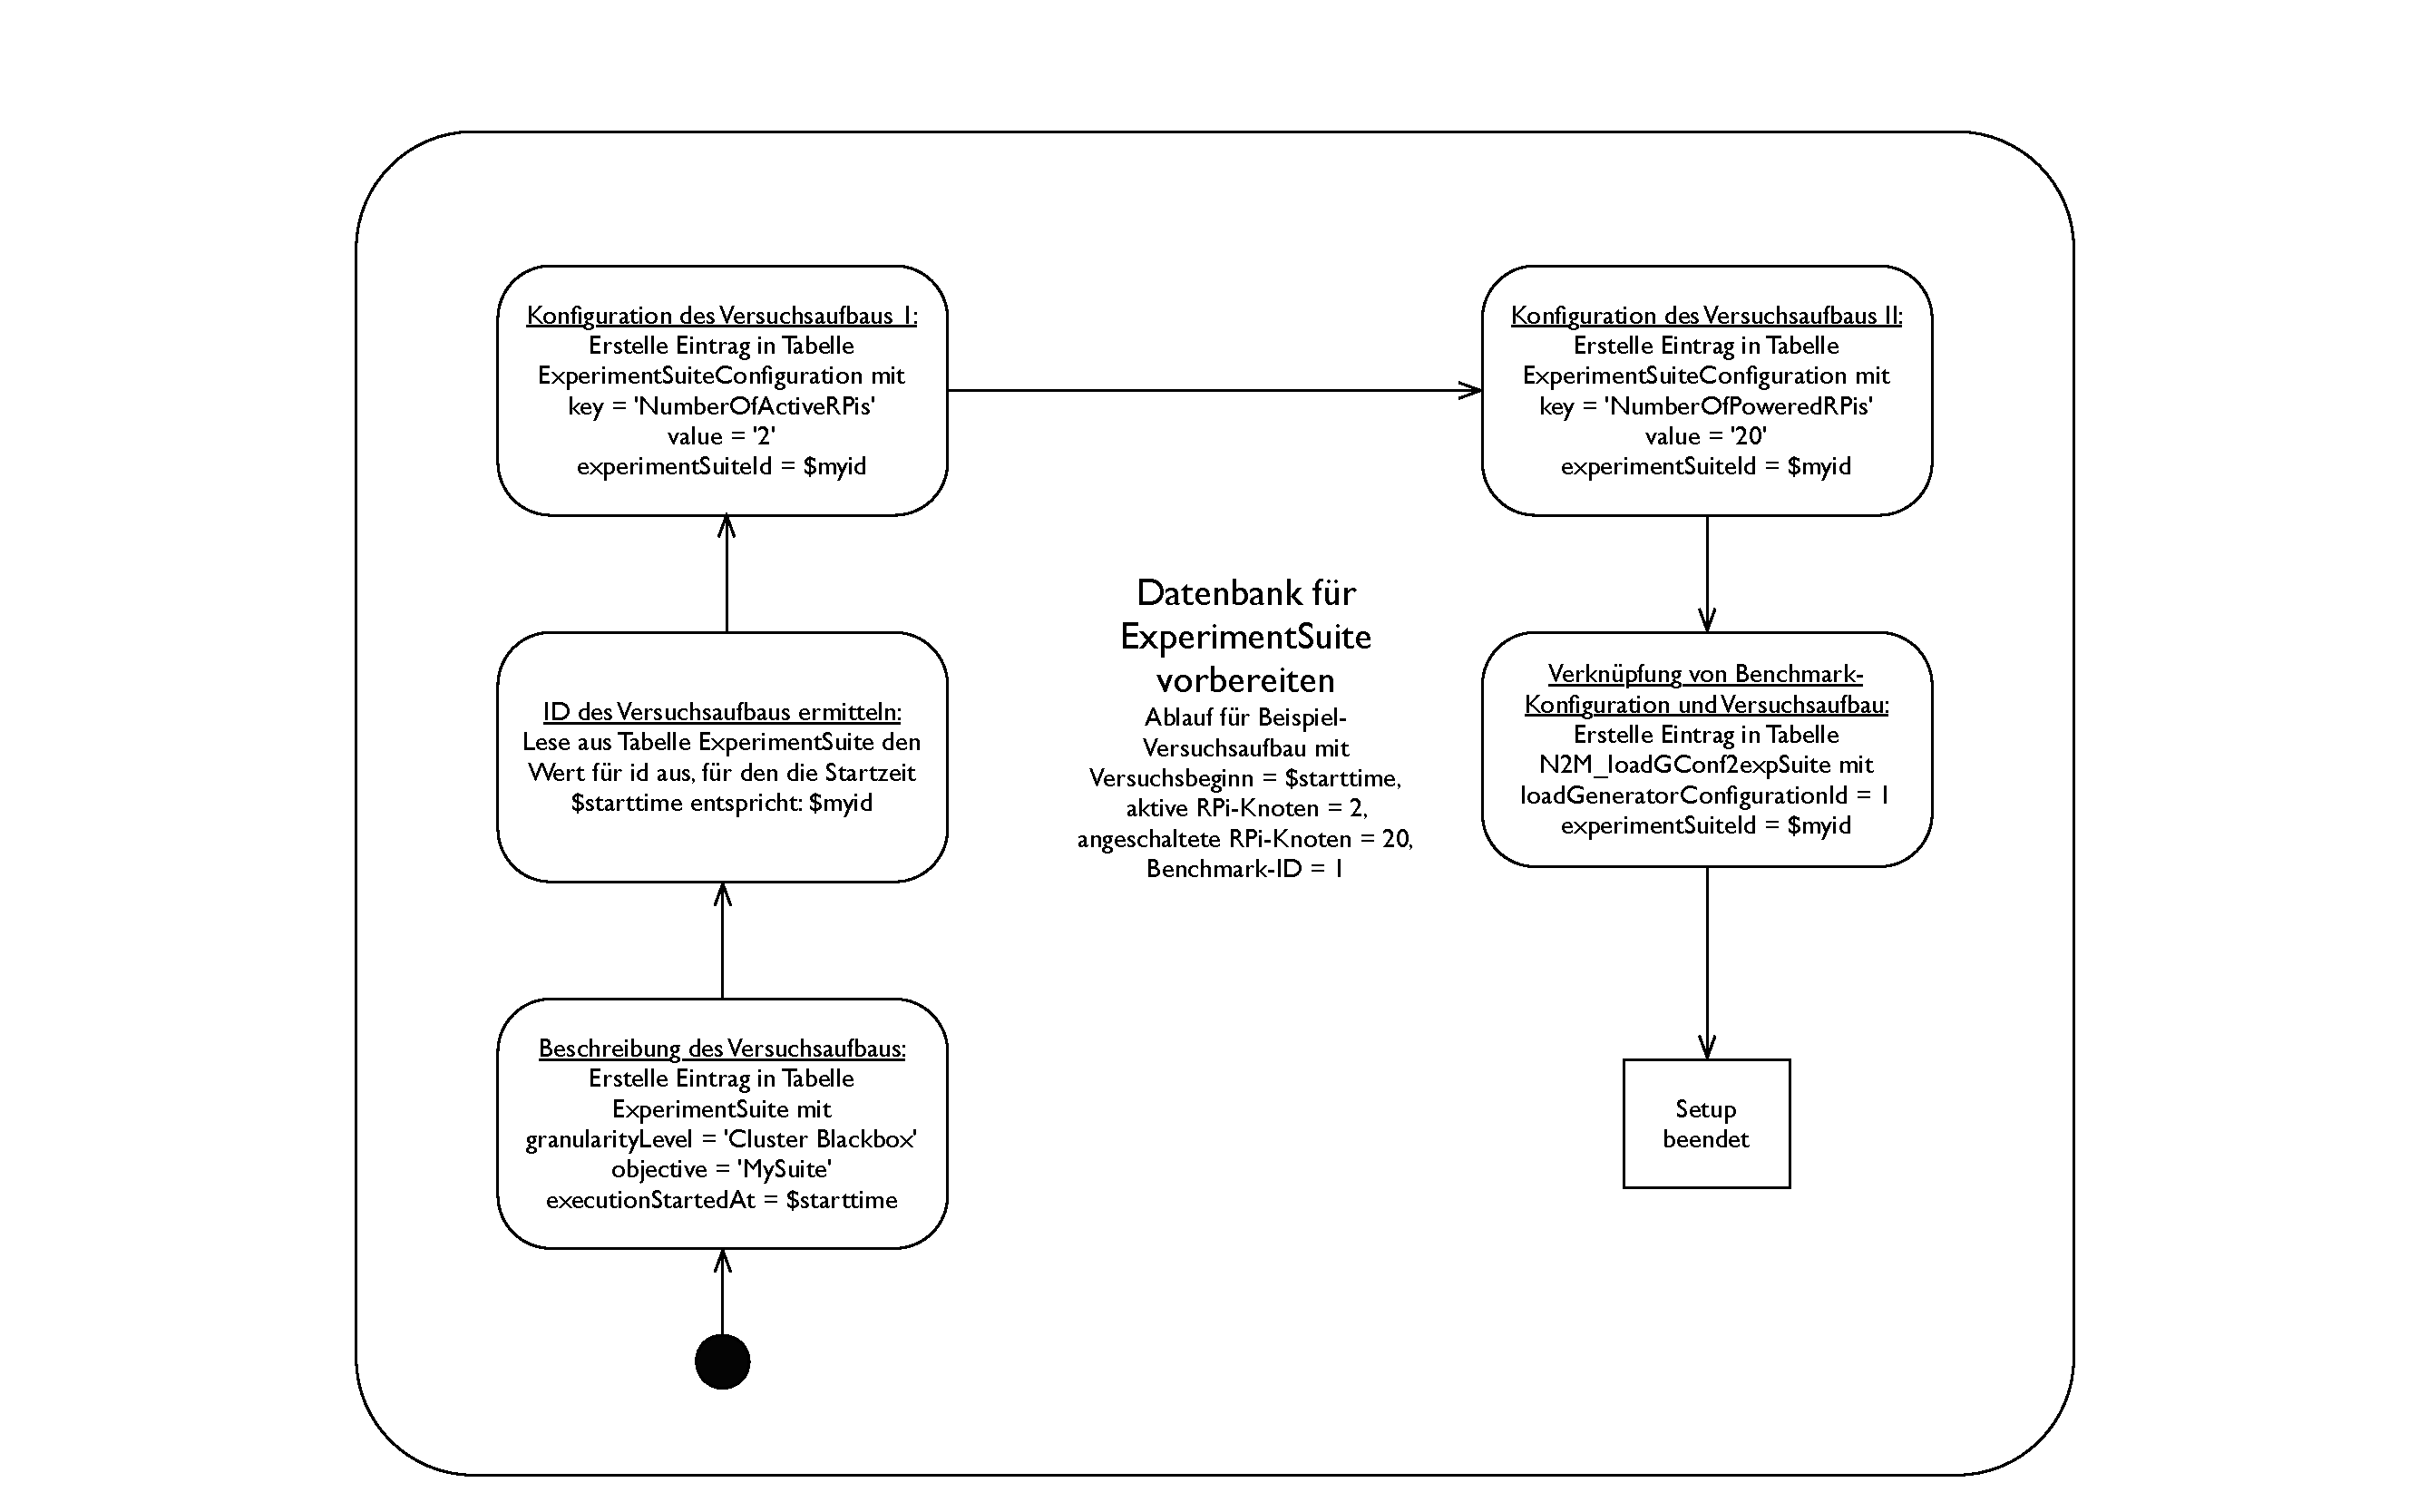
\includegraphics[scale=0.5]{dbconfig2.pdf}}
\caption{Aktivit"atsdiagramm zur Vorbereitung der Datenbank f"ur eine ExperimentSuite.}
\label{fig:Dbconfig2}
\end{figure}
			\textbf{\item Verteilte Ausf"uhrung des Benchmarks auf n RPi-Knoten.}\\ 
Die verteilte Ausf"uhrung eines Benchmark-Programms wird mit dem Befehl 
\begin{verbatim}
mpiexec -n -machinefile -wdir file 
\end{verbatim}
gestartet. Dabei spezifiziert \texttt{-n} die gew"unschte Anzahl an parallelen Programmaufrufen, \texttt{-machinefile} den Pfad zum Machinefile, \texttt{-wdir} das Verzeichnis, in das zur Ausf"uhrung des Programms gewechselt werden soll, und \texttt{file} die auszuf"uhrende Datei (vgl. \url{http://www.mpich.org/static/docs/latest/www1/mpiexec.html}). Ein Beispielaufruf zur parallelen Ausf"uhrung von HPLinpack auf vier RPi-Nodes mit der hier verwendeten Verzeichnisstruktur w"are also  
\begin{verbatim}
mpiexec -n 4 -machinefile /srv/libraries/etc/mpich-3.0.4-shared
/machinefile -wdir /srv/benchmarks/bin
/hpl-2.1 /srv/benchmarks/bin/hpl-2.1/xhpl
\end{verbatim}
			\textbf{\item Schreiben der Ergebnisdaten.}\\
Die Ausgabe des Benchmark-Programms wird in die vorbereitete Logdatei geschrieben. Falls das Programm in seiner Ausgabe keinen Zeitstempel vorsieht (z.B. STREAM), wird dieser ermittelt und der Ausgabe als zus"atzliche Zeile hinzugef"ugt. Das ist wichtig, damit sp"ater f"ur jeden Messwert ein Zeitstempel in die Datenbank eingegeben werden kann (vgl. Schritte d und e). Auch zum Abgleich der Messergebnisse der Benchmarks mit denen des Strommessger"ats ist ein Zeitstempel n"otig. % TODO: Verweis
		\end{enumerate}
		\textbf{\item Iteration "uber n RPi-Knoten:} 
		\begin{enumerate}\bfseries
			\item Einrichten der Datenbank.\\
\normalfont{Die Datenbank wird wie in Schritt b i beschrieben vorbereitet. Der wesentliche Unterschied zu Schritt ist der Wert f"ur die Anzahl angeschalteter RPi-Knoten. Es wird nicht mehr konstant 20 eingetragen, sondern n, da nicht mehr aktive RPi-Knoten heruntergefahren werden.} 
			\textbf{\item Verteilte Ausf"uhrung des Benchmarks auf n RPi-Knoten.}\\
Analog zu Schritt b ii.
			\textbf{\item Herunterfahren von RPi-Knoten n.}\\
Beim zweiten Lauf eines Benchmark-Programms auf n RPi-Knoten wird der nun nicht mehr ben"otigte bzw. aktive Knoten heruntergefahren. Das gilt nicht f"ur den Ausf"uhrungsknoten \texttt{pi03}, der bis zum Schluss des Experiments zur Ausf"uhrung der Skripte und Eingabe der Messergebnisse in die Datenbank verwendet wird. 
			\textbf{\item Schreiben der Ergebnisdaten.}\\ 
Analog zu Schritt b iii.
		\end{enumerate}
		\textbf{\item Parsen der Logdateien f"ur die Datenbank-Eingabe.}\\
Die Ausgabe der Benchmarks ist h"ochst unterschiedlich und entspricht nat"urlich nicht dem Eingabeformat f"ur die Datenbank \texttt{rpiWerte}. Daher wird pro ausgef"uhrtem Benchmark eine Eingabedatei f"ur die Datenbank erstellt, die pro ExperimentSuite eine Zeile mit den Messergebnissen und Zeitstempel enth"alt, getrennt durch Leerzeichen. So enth"alt z.B. eine Zeile einer Datenbank-Eingabedatei f"ur STREAM: 
\begin{verbatim}
Copy: 3649.3 0.167595 0.166607 0.168846 Scale: 3428.0 0.178749 
0.177361 0.180439 Add: 4749.8 0.192614 0.192010 0.193745 Triad: 
4630.1 0.197780 0.196974 0.199436 Unixtime: 1396608095
\end{verbatim} 
Eine Beispielzeile einer Datenbank-Eingabedatei f"ur HPLinpack: 
\begin{verbatim}
WR00L2L2 29 1 2 2 0.09 1.965e-04 HPL_pdgesv() end time Wed Mar 
26 15:39:05 2014
\end{verbatim} 
		\textbf{\item Schreiben der Messergebnisse in die Datenbank.}\\
Falls die Zeitstempel in der Datenbank-Eingabedatei noch nicht dem Format des Unix-Zeitstempels UTC entsprechen (vergangene Sekunden seit dem 1. Januar 1970, vgl. \url{http://unixhelp.ed.ac.uk/CGI/man-cgi?date}) wie z.B. bei HPLinpack (vgl. Schritt d), werden sie in dieses Format konvertiert. F"ur jeden Messwert muss ein Eintrag in der Tabelle \texttt{MeasurementValue} mit Werten f"ur Parameter, Messwert und Zeitstempel erstellt werden. 		
	\end{enumerate}
\end{enumerate}
\noindent
Zur Durchf"uhrung dieser Schritte wurden drei Shellskripte erstellt: \texttt{startBenchmarks.sh} zum Erstellen des Machinefile, Einh"angen des geteilten Verzeichnisses und Aufruf der Skripte \texttt{STREAM.sh} und \texttt{hpl-2.1.\-sh} (Schritte 1--3). Schritt 4 wird f"ur den jeweiligen Benchmark durch die Shellskripte \texttt{STREAM.sh} und \texttt{hpl-2.1.sh} ausgef"uhrt, die von \texttt{startBenchmarks.sh} aufgerufen werden. 

\section{Strommessung}
% Name, Beschreibung
Die Messung des Stromverbrauchs erfolgt mit dem Strommessger"at \textit{Energenie EGM-PWM-LAN} (vgl. \url{http://energenie.com/item.aspx?id=6736&lang=de}), im Folgenden als \textit{Energenie} bezeichnet. Es wird zwischen die Steckdose und den Bramble gesteckt und "uber ein LAN-Kabel mit dem Netzwerk verbunden. 

% Aktivierung
F"ur den Versuchsaufbau war dem Energenie eine statische IP-Adresse zugewiesen und ein DNS-Eintrag erstellt worden. Damit ist es m"oglich, im lokalen Netzwerk auf das Ger"at und die ermittelten Messwerte zuzugreifen. F"ur den Zugriff gibt es mehrere M"oglichkeiten, darunter eine Webbrowser- und eine Windows-Anwendung. Damit die Software das Ger"at erkennt, muss es sich im selben Subnetz befinden wie der zugreifende Rechner. 

Die Software musste einmalig f"ur die Benutzung des Energenie eingerichtet werden. Dazu wurden nach der Installation des Programms \textit{PowerManager} IP-Adresse und ein Name f"ur das Energenie eingetragen. In der Webbrowser-Anwendung wurde das Standardpasswort ge"andert und die NTP-Zeitsynchronisation aktiviert. 

% Messgrößen 
Das Energenie misst Spannung in Volt, elektrischen Strom in Amp\`{e}re, Leistung in Watt und Arbeit in Kilowattstunden. Die Messgenauigkeit innerhalb des Messbereichs von $50 W - 2500 W$ betr"agt $\pm 2\%$ bzw. $\pm 1 W$ (vgl. \cite{scrguide03}). % TODO Messfehler ermitteln 

% Datenzugriff 
F"ur den Versuchsaufbau erwies sich die Webbrowser-Anwendung als weniger geeignet, da sie haupts"achlich Konfigurationsfunktionen bietet. Zwar werden auf einer grafischen Oberfl"ache die jeweils aktuellen Werte f"ur Spannung, elektrischen Strom, Leistung und Arbeit angezeigt, doch es k"onnen keine Messwerte f"ur eine Zeitspanne abgerufen werden. 

Das Programm PowerManager bietet erweiterte Funktionalit"aten, z.B. die Visualisierung der Leistung "uber eine Zeitspanne als Kurve. Die ermittelten Messwerte bei Ausf"uhrung des Programms in einer SQLite-Datenbank \texttt{database.sqlite} im Verzeichnis \texttt{C:\textbackslash Program Data\textbackslash PowerManagerDatabase} auf der zugreifenden Windows-Maschine abgelegt. Sie k"onnen auch als xls-Datei exportiert werden. Dabei werden pro Messung drei Werte angegeben: Beginn der Messung, Ende der Messung und Leistung in Watt. In der Datenbank werden f"ur jede Messung zus"atzliche Werte abgelegt wie Widerstand in Ohm und Frequenz in Hertz. F"ur die ExperimentSuites sind die Eintr"age \texttt{Stamp} (Zeitstempel als Integer-Wert) und \texttt{P} (Leistung in Watt als Double-Wert) in der Tabelle \texttt{LogValues} entscheidend. Die Entscheidung f"ur das Auslesen der SQLite-Datenbank gegen"uber dem xls-Export fiel wegen der h"oheren Granularit"at der Zeitstempel. 

% Setup für ExperimentSuite 
Das Aktivit"atsdiagramm \ref{fig:energenie} zeigt, welche Schritte aus Benutzersicht pro ExperimentSuite f"ur die Strommessung notwendig sind: 
\begin{figure}[htb]
  \centering
  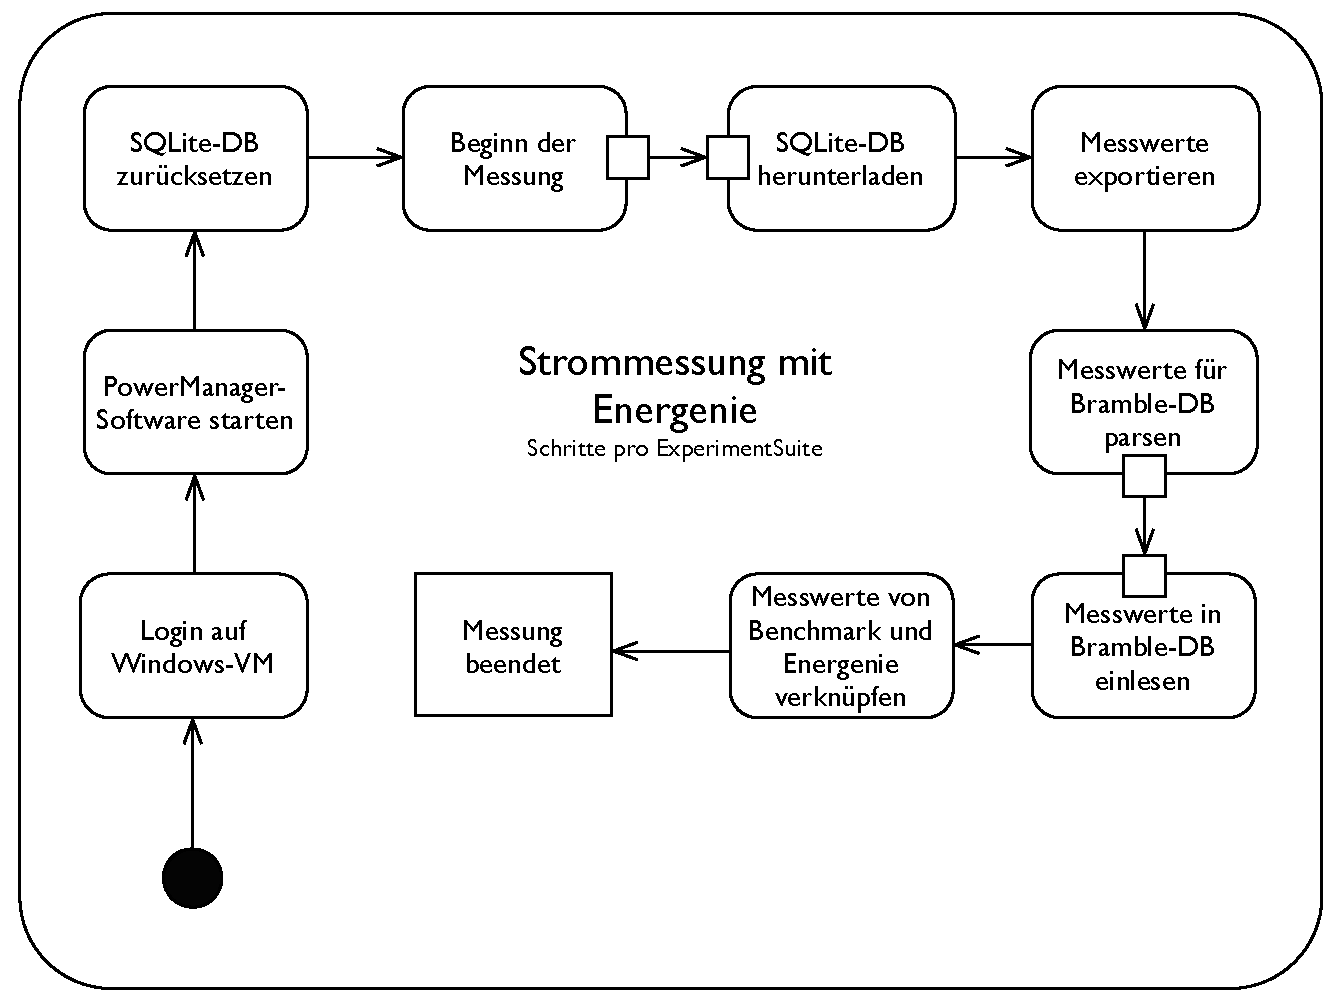
\includegraphics[scale=0.7]{energenie.pdf}\\ 
  \caption{Aktivit"atsdiagramm zur Durchf"uhrung einer Strommessung f"ur eine ExperimentSuite.}
  \label{fig:energenie}		
\end{figure}
\begin{enumerate}\bfseries
% Login auf VM 
	\item Login auf Windows-Maschine.\\
\normalfont
Das Programm PowerManager wird nur f"ur ein Windows-Betriebssystem (Windows XP oder h"oher) angeboten. F"ur die Ausf"uhrung war eine virtuelle Windows-Maschine (Windows 7) im lokalen Netzwerk zur Verf"ugung gestellt worden. 
% PowerManager starten 
	\textbf{\item Start der PowerManager-Software.}
% Datenbank leeren 
	\textbf{\item Zur"ucksetzen der SQLite-Datenbank.}\\
Um m"oglichst wenige Messwerte zu erhalten, die nicht zur aktuellen ExperimentSuite geh"oren, ist es sinnvoll, die Datenbank jeweils vor dem Start einer ExperimentSuite zur"uckzusetzen. Die Aufzeichnung der Messwerte erfolgt st"andig und muss nicht gesondert angesto\ss en werden, solange das Energenie an den Bramble angeschlossen und die Anwendung aktiv ist. 
% Grafische Aufzeichnung starten (optional)
	\textbf{\item Start der grafischen Aufzeichnung.}\\ 
Optional ist es m"oglich, die aktuellen Messwerte f"ur die Leistung auf einer grafischen Oberfl"ache anzeigen zu lassen. Es hat sich zur "Uberwachung der Messung als sinnvoll erwiesen.
% SQLite-DB herunterladen 
	\textbf{\item Herunterladen der SQLite-Datenbank.}\\ 
Zur weiteren Verarbeitung der Messwerte muss die SQLite-Datenbank von der Windows-Maschine heruntergeladen werden.
% Export der Messwerte
	\textbf{\item Export der Messwerte.}\\
Zur weiteren Verarbeitung der Messwerte wird die Tabelle \texttt{LogValues} exportiert.
% Messwerte parsen für MySQL-DB rpiWerte
	\textbf{\item Parsen der Messwerte f"ur die Bramble-Datenbank.}\\
Zum Einlesen der Messwerte in die MySQL-Datenbank auf dem Bramble m"ussen sie in ein passendes Format gebracht werden. Hierf"ur wurde ein Shellskript \texttt{parseEnergyValues.sh} erstellt. Es erstellt eine Eingabedatei, die jeweils eine Zeile pro Messung mit Unix-Zeitstempel und Leistung enth"alt.
	\textbf{\item Einlesen der Messwerte in die Bramble-Datenbank.}\\
F"ur jede Messung muss ein Eintrag in der Tabelle \texttt{MeasurementValue} mit Werten f"ur Parameter, Messwert, Zeitstempel und der ID des Strommessger"ats erstellt werden. Da die MySQL-Datenbank auf dem Bramble liegt, wurde hierf"ur ein Shellskript \texttt{writeEnergyValues.sh} im Verzeichnis \texttt{/home/rpi-user/experimentsuite} auf dem Bramble erstellt. 
% Messwerte von Strommessung und Benchmarks matchen 
	\textbf{\item Verkn"upfung der Messwerte von Energenie und Benchmark-Programm.}\\ 
Im letzten Schritt m"ussen die Messwerte von Energenie und Benchmark-Programm f"ur die jeweilige ExperiementSuite verkn"upft werden. Hierzu wurde ein Shellskript \texttt{matchEnergyValues.sh} im selben Verzeichnis auf dem Bramble erstellt. 
\end{enumerate}

\section{Ergebnisse}\label{Ergebnisse}

Der folgende Abschnitt pr"asentiert die Untersuchungsergebnisse f"ur HPLinpack und STREAM auf dem Bramble. Jeder Benchmark wurde zweimal ausgef"uhrt. Bei Messreihe 1 waren alle RPi-Knoten angeschaltet, bei Messreihe 2 wurden nicht mehr aktive Knoten heruntergefahren. \texttt{pi03} als Berechnungsknoten blieb immer angeschaltet (vgl. Kap. \ref{Versuchsaufbau}).

Da keine Implementierung von Whetstone f"ur eine verteilte Berechnung auf Raspbian existiert, war im Verlauf der Untersuchung vorgegeben worden, Whetstone nicht zu ber"ucksichtigen. HPLinpack in der verwendeten Implementierung ben"otigt mindestens vier CPUs oder parallele Prozesse. Hier wurde jeder CPU, d.h. jedem RPi-Knoten, genau ein Prozess zugewiesen, sodass zur Ausf"uhrung von HPLinpack mindestens vier angeschaltete und aktive RPi-Knoten ben"otigt werden. 

Zur besseren Vergleichbarkeit wurde die verteilte Ausf"uhrung von STREAM daran angepasst, d.h. auch STREAM wurde auf mindestens vier RPi-Knoten parallel ausgef"uhrt. 

\subsection{HPLinpack: Performance}\label{Ergebnisse-HPL}

HPLinpack in der verwendeten Implementierung (vgl. Kap. \ref{Linpack-RPi}) liefert folgende Ausgabe:

Zun"achst erfolgt eine Erl"auterung der verwendeten Eingabe- und Ausgabeparameter. Ein Teil der Eingabeparameter ist invariabel (\texttt{eps} bzw. Maschinengenauigkeit und \texttt{T/V} bzw. Ausf"uhrungszeit). Die anderen Eingabeparameter sind in der Datei \texttt{HPL.dat} angegeben, die im selben Verzeichnis wie die ausf"uhrbare Datei des Benchmark-Programms liegen muss. Dazu z"ahlen die Problemgr"o\ss e bzw. Ordnung des zu l"osenden linearen Gleichungssystems \texttt{N}, die Anzahl an verwendeten Problemgr"o\ss en \texttt{\#N}, die Blockgr"o\ss e\texttt{NB}\footnote{Die L"osung des linearen Gleichungssystems erfolgt mittels L/U-Faktorisierung. Dazu wird zun"achst eine $n\times n+1$-Koeffizientenmatrix der Ausgangsmatrix A erzeugt. Diese wird zur weiteren Bearbeitung in Bl"ocke der Gr"o\ss e $NB\times NB$ aufgeteilt.} und die Gr"o\ss e des Prozessorennetzes (\texttt{P} und \texttt{Q})\footnote{Die Bl"ocke werden zur Bearbeitung einem Netz aus Prozessoren "ubergeben der Gr"o\ss e $P\times Q$ "ubergeben. \texttt{P} bezeichnet darin die Anzahl von Prozessoren in einer Spalte, \texttt{Q} die Anzahl von Prozessoren in einer Zeile des Netzes.} (vgl. \url{http://www.netlib.org/benchmark/hpl/algorithm.html}). 

Die Ausgabeparameter sind invariabel. Die wichtigsten davon sind \texttt{Gflops} (Ausf"uhrungsrate in GFLOPs) und \texttt{Time} (Ausf"uhrungsdauer in Sekunden). F"ur jede Ausf"uhrung von HPLinpack werden 864 Tests durchgef"uhrt, d.h. 864 Messwerte f"ur Ausf"uhrungsrate und Ausf"uhrungsdauer erzeugt. \texttt{Gflops} wird auf 8, \texttt{Time} auf 2 Nachkommastellen genau angegeben. 

Die Diagramme \ref{fig:hpl1} und \ref{fig:hpl2} zeigen die Ergebnisse von Messreihe 1, jeweils skaliert auf 16--4 RPi-Knoten. Dabei sind jeweils n RPi-Knoten aktiv und alle 20 RPi-Knoten angeschaltet.
\begin{figure}[htb]
  \centering
  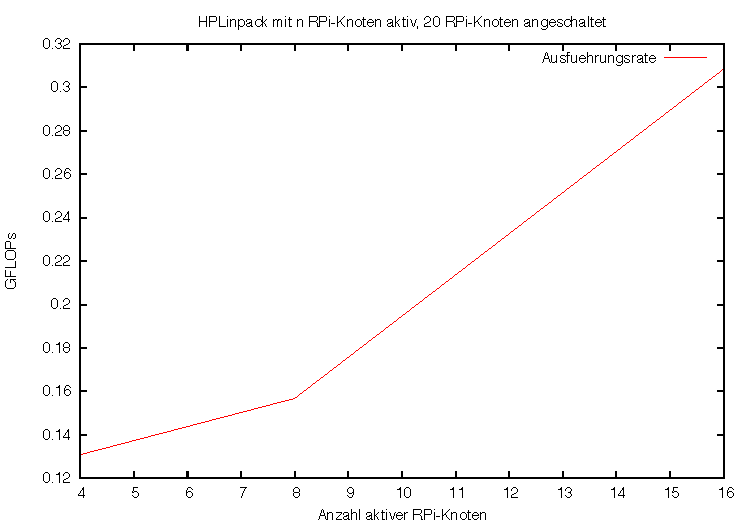
\includegraphics[scale=0.8]{hpl1.pdf}\\ 
  \caption{Ausf"uhrungsrate f"ur HPLinpack, Messreihe 1.}
  \label{fig:hpl1}		
\end{figure}
\begin{figure}[htb]
  \centering
  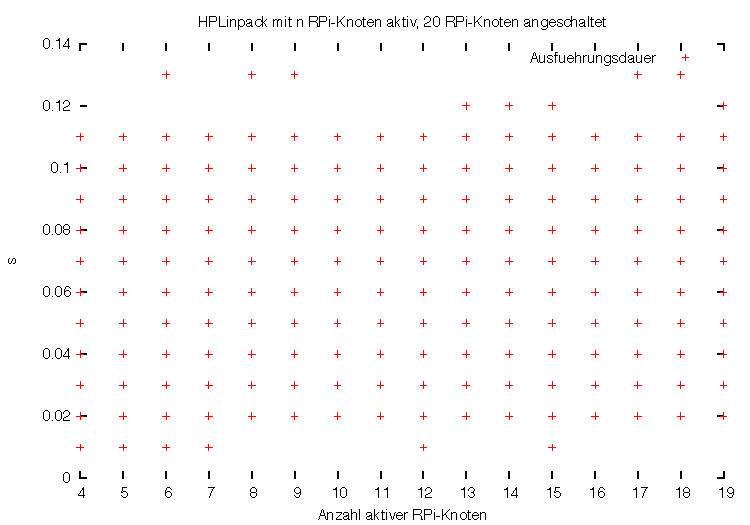
\includegraphics[scale=0.8]{hpl2.pdf}\\ 
  \caption{Ausf"uhrungsdauer f"ur HPLinpack, Messreihe 1.}
  \label{fig:hpl2}		
\end{figure}
\noindent
Die Diagramme \ref{fig:hpl5} und \ref{fig:hpl6} stellen die Ergebnisse von Messreihe 1 denen von Messreihe 2 gegen"uber, in der nicht mehr aktive RPi-Knoten nach der Ausf"uhrung des Benchmarks heruntergefahren werden. Die Ergebnisse von Messreihe 1 sind rot, die von Messreihe 2 blau dargestellt.
\begin{figure}[htb]
  \centering
  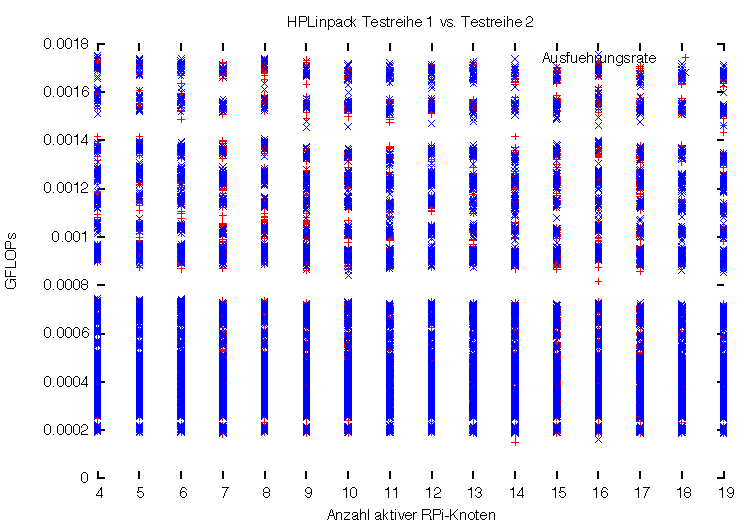
\includegraphics[scale=.8]{hpl5.pdf}\\ 
  \caption{Ausf"uhrungsrate f"ur HPLinpack, Messreihe 1 und Messreihe 2.}\label{fig:hpl5}
\end{figure}
\begin{figure}[htb]
  \centering
  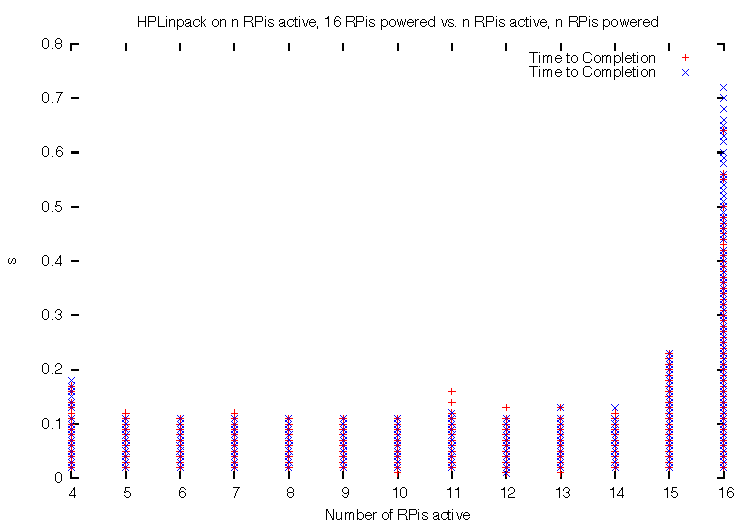
\includegraphics[scale=.8]{hpl6.pdf}\\ 
  \caption{Ausf"uhrungsdauer f"ur HPLinpack, Messreihe 1 und Messreihe 2.}\label{fig:hpl6}
\end{figure}
\subsection{STREAM: Performance}\label{Ergebnisse-Stream}

In der Ausgabe von STREAM werden zun"achst ebenfalls die verwendeten Parameter angegeben, darunter Anzahl an Prozessoren, Vektorl"ange, Speicherbedarf und Anzahl an Iterationen f"ur jedes Modul. F"ur die vier Module Copy, Scale, Add und Triad (vgl. Kap. \ref{Funktion-STREAM}) werden die beste erzielte Ausf"uhrungsrate in MB/s (\texttt{Rate}) und die durchschnittliche (\texttt{Avg time}), minimale (\texttt{Min time}) und maximale Ausf"uhrungsdauer (\texttt{Max time}) in Sekunden ausgegeben. Die Ausf"uhrungsrate wird auf eine, die Ausf"uhrungsdauer auf 6 Nachkommastellen genau angegeben. 

Diagramme \ref{fig:stream1} und \ref{fig:stream2} zeigen die Ergebnisse von Messreihe 1 f"ur STREAM. Ausgabeparameter sind Ausf"uhrungsrate in MB/s und durchschnittliche Ausf"uhrungsdauer in Sekunden f"ur Copy, Scale, Add und Triad, skaliert auf 16--4 RPi-Knoten. Dabei sind jeweils n RPi-Knoten aktiv und alle 20 RPi-Knoten angeschaltet.  
%\begin{figure}[htb]
%  \centering
%  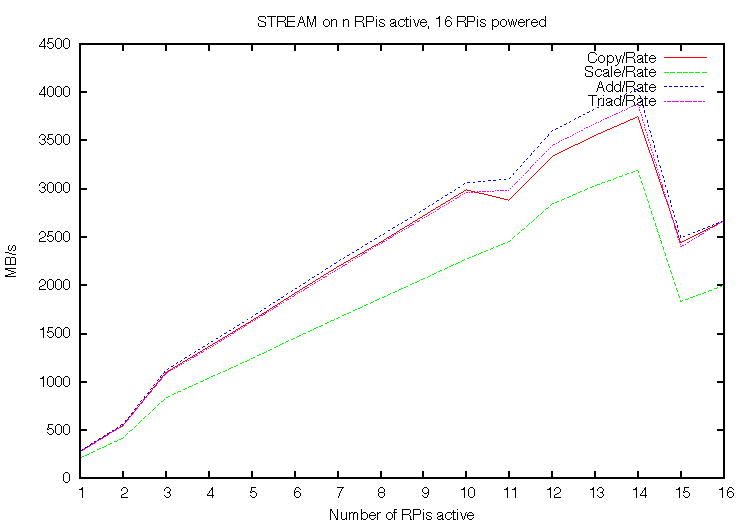
\includegraphics[scale=0.8]{stream1.pdf}\\ 
%  \caption{Ausf"uhrungsrate f"ur STREAM, Messreihe 1.}
%  \label{fig:stream1}		
%\end{figure}
%\begin{figure}[htb]
%  \centering
%  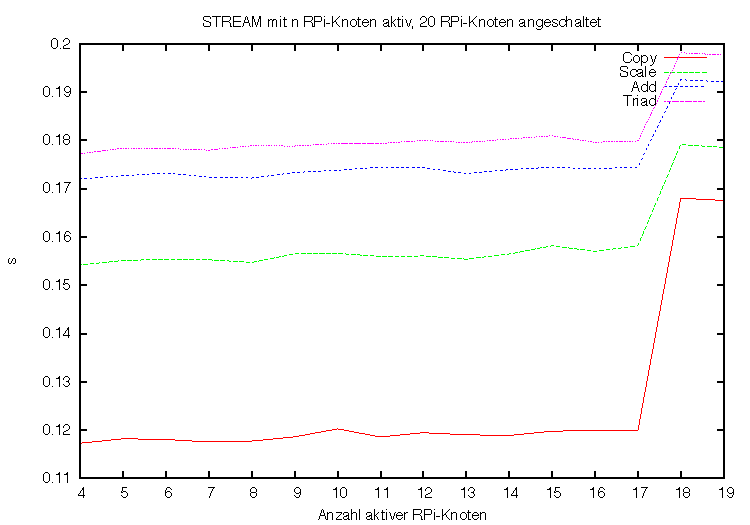
\includegraphics[scale=0.8]{stream2.pdf}\\ 
%  \caption{Ausf"uhrungsdauer f"ur STREAM, Messreihe 1.}
%  \label{fig:stream2}		
%\end{figure}
\noindent
Die Diagramme \ref{fig:stream5} und\ref{fig:stream6} stellen die Ergebnisse von Messreihe 1 und Messreihe 2 f"ur STREAM gegen"uber. Die Ergebnisse von Messreihe 1 sind rot, die Ergebnisse von Messreihe 2 sind blau markiert. 
%\begin{figure}[htb]
%  \centering
%  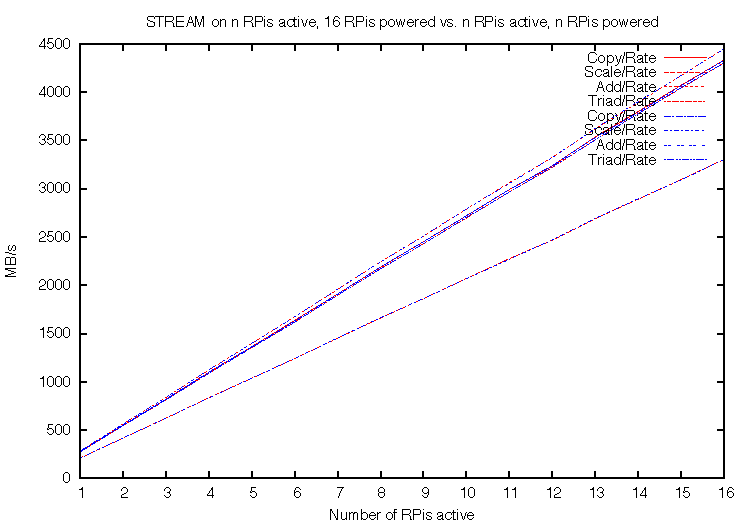
\includegraphics[scale=.8]{stream5.pdf}\\ 
%  \caption{Ausf"uhrungsrate f"ur STREAM, Messreihe 1 und Messreihe 2.}\label{fig:stream5}
%\end{figure}
%\begin{figure}[htb]
%  \centering
%  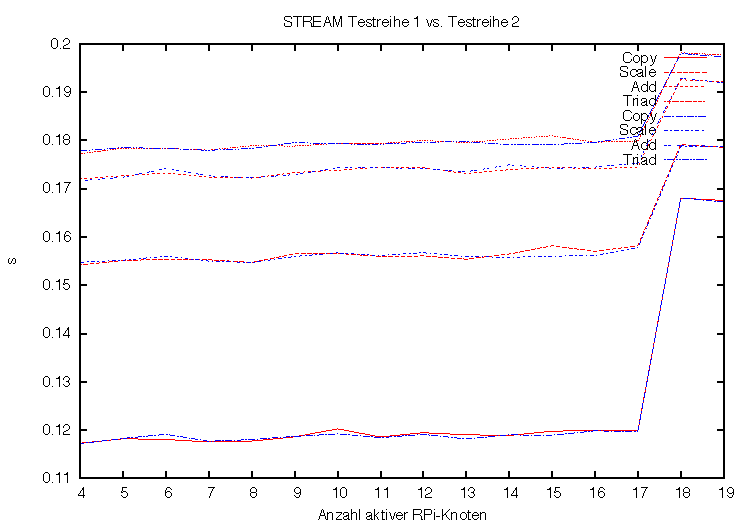
\includegraphics[scale=.8]{stream6.pdf}\\ 
%  \caption{Ausf"uhrungsdauer f"ur STREAM, Messreihe 1 und Messreihe 2.}\label{fig:stream6}
%\end{figure}

\subsection{Stromverbrauch}\label{Ergebnisse-Energenie}

Die Diagramme \ref{fig:strom1} und \ref{fig:strom2} zeigen die Ergebnisse der Strommessung f"ur HPLinpack. Diagramm \ref{fig:strom1} zeigt den Stromverbrauch bei der Ausf"uhrung auf 19 -- 1 RPi-Knoten, wobei alle 20 RPi-Knoten angeschaltet sind (Messreihe 1). Diagramm \ref{fig:strom2} zeigt den Stromverbrauch, wenn nicht mehr aktive RPi-Knoten heruntergefahren werden (Messreihe 2). 
%\begin{figure}[htb]
%  \centering
%  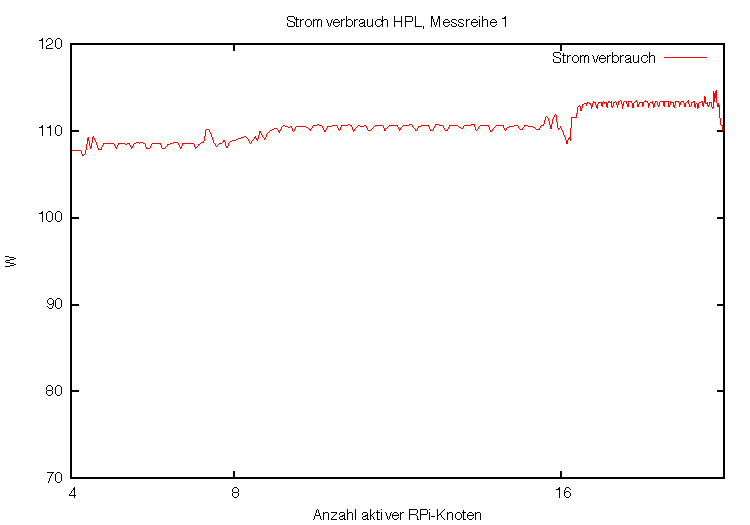
\includegraphics[scale=.8]{strom1.pdf}\\ 
%  \caption{Stromverbrauch in W f"ur HPLinpack, Messreihe 1.}\label{fig:strom1}
%\end{figure}
%\begin{figure}[htb]
%  \centering
%  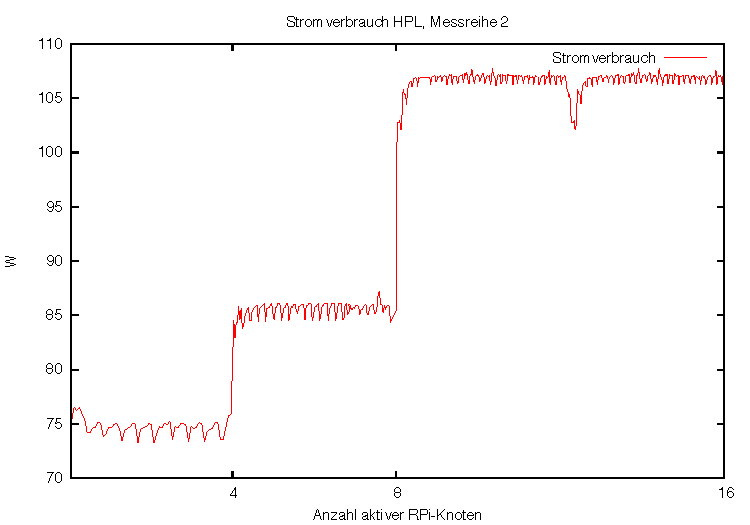
\includegraphics[scale=.8]{strom2.pdf}\\ 
%  \caption{Stromverbrauch in W f"ur HPLinpack, Messreihe 2.}\label{fig:strom2}
%\end{figure}
\noindent
Die Diagramme \ref{fig:strom3} und \ref{fig:strom4} zeigen analog die Ergebnisse der Strommessung f"ur STREAM. Diagramm \ref{fig:strom3} zeigt den Stromverbrauch bei der Ausf"uhrung auf 19 -- 4 RPi-Knoten, wobei alle 20 RPi-Knoten angeschaltet sind (Messreihe 1). Diagramm \ref{fig:strom4} zeigt den Stromverbrauch, wenn nicht mehr aktive RPi-Knoten heruntergefahren werden (Messreihe 2).
%\begin{figure}[htb]
%  \centering
%  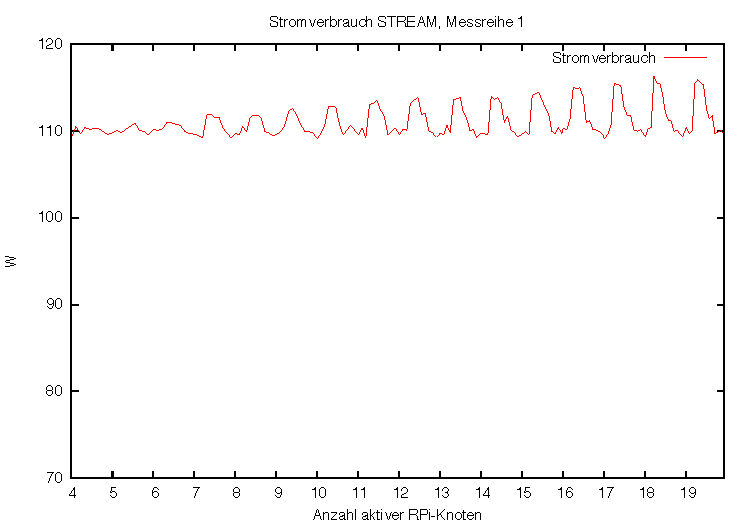
\includegraphics[scale=.8]{strom3.pdf}\\ 
%  \caption{Stromverbrauch in W f"ur STREAM, Messreihe 1.}\label{fig:strom3}
%\end{figure}
%\begin{figure}[htb]
%  \centering
%  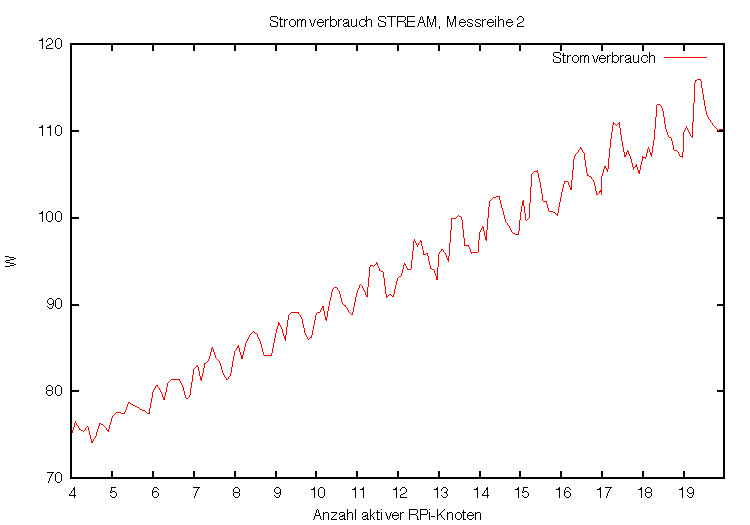
\includegraphics[scale=.8]{strom4.pdf}\\ 
%  \caption{Stromverbrauch in W f"ur STREAM, Messreihe 2.}\label{fig:strom4}
%\end{figure}
\endinput 


